\documentclass[thesis-solanki.tex]{subfiles}


\ifMain
\externaldocument{thesis-solanki}
\fi
\begin{document}

\chapter{Prototype 2}{\label{proto2}}

\section{About this chapter}
This chapter attempts to infuse the generic methodology from Chapter~\ref{proto1} in a current \progLang{Prolog}
implementation \cite{prolog-lib} and make the unification ``monadic''.

This chapter discusses the idea of implementing a basic working \progLang{Prolog} query resolver while using \codeLibrary{prolog-0.2.0.1}
\cite{prolog-lib} as the base implementation.
The language modifications and unification mechanism have been taken from Chapter~\ref{proto1} and adapted to fit
in with the other components such as the search strategy of the library.


\section{How \protect\codeLibrary{prolog-0.2.0.1} works}

The \codeLibrary{prolog-0.2.0.1} library (\cite{prolog-lib}) was written by Matthias Bartsch and consists of 14 \progLang{Haskell} files. It 
implements data base assertions and cuts but lacks any IO facilities. Moreover, the abstract syntax used to implement the language is rigid
and leaves very little to no scope for extension. Figure~\ref{fig:prlg0201architecture} describes its architecture.

\begin{figure}[H]
\centering
\includegraphics[scale = .6]{prolog0201_architecture.png}
\caption{\codeLibrary{prolog-0.2.0.1} \cite{prolog-lib} architecture}
\label{fig:prlg0201architecture}
\end{figure}


\begin{comment}

As described in the previous chapter about extending languages to incorporate functionality, this prototype applies
the procedure to the eDSL in \cite{prolog-lib}.
\end{comment}

From the Listing~\ref{tab:origgramp0201} we will focus on \haskellConstruct{Terms}, since the others just
add wrappers around expressions which can be created by it.
This language suffers from most of the problems discussed in the previous chapter.
The above is used to construct \progLang{Prolog} ``terms'' which are of a ``single type''.

The implementation consists of components that one would find in a language processing system (see
Figure~\ref{fig:A language-processing system}).



\begin{figure}[H]
\centering
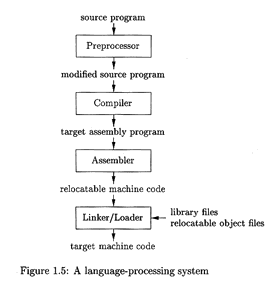
\includegraphics[scale = .95]{Language_Processing_System.png}
\caption{A language-processing system (taken from \cite{Aho:1986:CPT:6448})}
\label{fig:A language-processing system}
\end{figure}

They specifically contain parts of a compiler (see Figure~\ref{fig:Phases of Compiler}).

\begin{figure}[H]
\centering
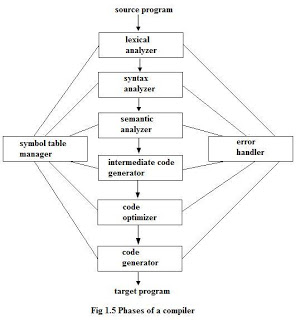
\includegraphics[scale = 0.7]{Phases_of_compiler.jpg}
\caption{Phases of Compiler \cite{Aho:1986:CPT:6448}}
\label{fig:Phases of Compiler}
\end{figure}

The architecture for a compiler as described in Figure~\ref{fig:Phases of Compiler} is not needed since
\progLang{Haskell} provides most of them.
Nonetheless, the library has the following major components as shown in Figure~\ref{fig:prlg0201architecture}:

\begin{itemize}
\item the syntax which defines the language,

\item the database which stores the expressions and language constructs,

\item the parser,

\item the interpreter,

\item the unifier,

\item the Read-Eval-Print Loop (REPL).
\end{itemize}

To prove the modularity of the approach used in Chapter~\ref{proto1} for language modification and monadic unification only the abstract syntax and unifier will be customized.

\section{What we do in this prototype?}

Figure~\ref{fig:architecture-proto-2} describes the components of this implementation and the relation between them.

\begin{figure}[H]
  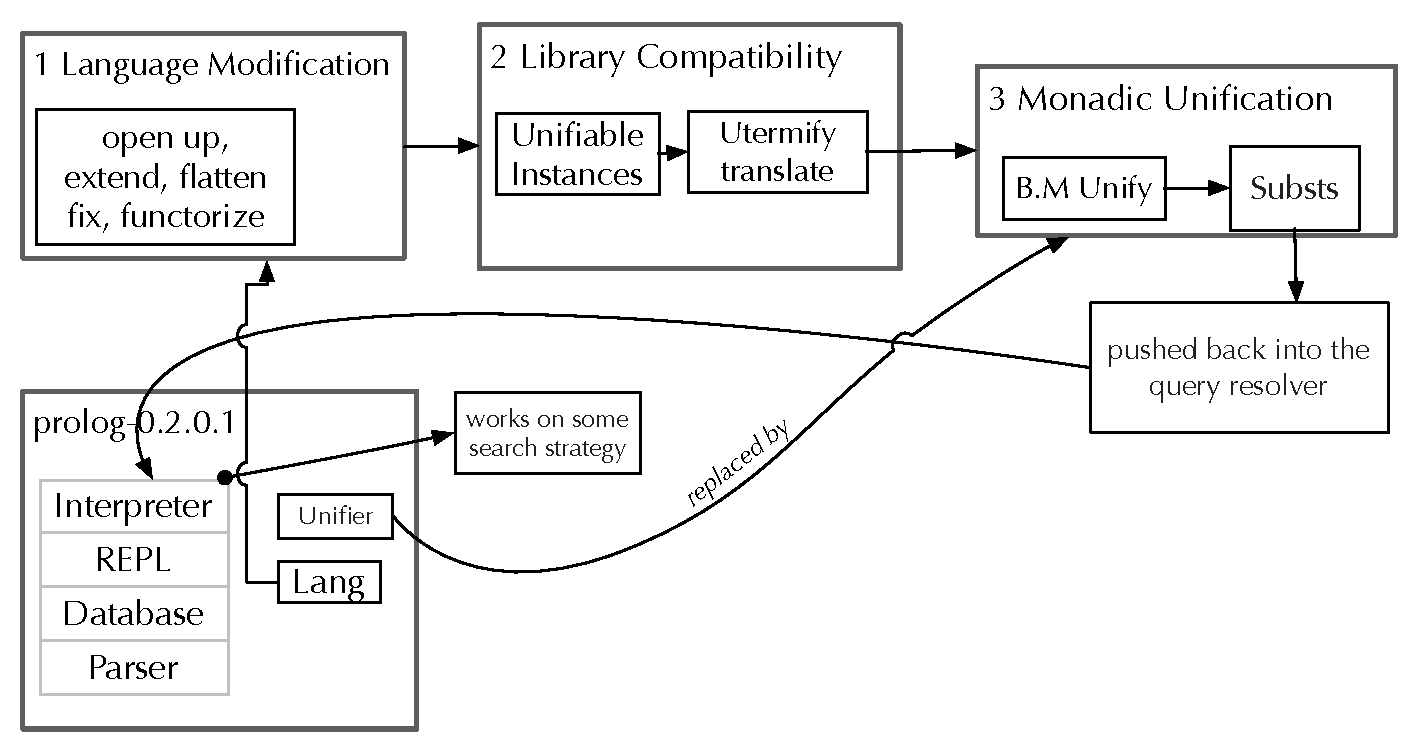
\includegraphics[width=1\textwidth]{Prototype-2-diagram.pdf}
\vspace*{-1cm}
  \caption{Architecture of Prototype 2}
  \label{fig:architecture-proto-2}
\end{figure}


Unification is a part of how \progLang{Prolog} works to produce a solution to the query. The \prologConstruct{unification} procedure
tells us whether or not two terms can be made equal. Before reaching that state, two terms must be gathered depending 
upon matching rules in the knowledge base. This is where a search strategy comes into play along with a backtracking mechanism.

Putting everything together forms the \progLang{Prolog} query resolver.
Given a query and a knowledge, the query resolver matches the input query with the rules in the knowledge base to
create a list of goals to satisfy to generate an unifier along with saving choice points on the way for
backtracking.

This chapter discusses how the abstract syntax and query resolver from \cite{prolog-lib} can be adapted to
the concepts and implementation from Chapter~\ref{proto1}.
This not only proves how generic and modular the approach from the previous chapter is, but also the working \progLang{Prolog} system
as a whole.



\section{Steps involved / Procedure}


\subsection{Flatten the language by introducing a type variable}
The first component describes the process of creating a modified version of the current abstract syntax used by the library as shown in Listing~\ref{tab:origgramp0201}.

\begin{code-list}[H]
	\begin{singlespace}
	\inputminted[linenos]{haskell}{haskell-proto2-original-grammar.hs}
	\end{singlespace}
	\caption{Original Recursive Grammar}
\label{tab:origgramp0201}
\end{code-list}

The grammar suffers from most of the drawbacks mentioned in Chapter~\ref{proto1}. This implementation focuses on creating a working  
\progLang{Prolog} query resolver with \haskellConstruct{monadic} \prologConstruct{uni\-fi\-ca\-tion}. The base implementation 
adopted from \codeLibrary{prolog-0.2.0.1} \cite{prolog-lib} already has a working implementation, but lacks benefits achieved from
our approach mention in the previous chapter.

The non-recursive implementation described in Listing~\ref{tab:flatgrp0201} introduces a type variable which separates the structure from 
the data itself.

\begin{code-list}[H]
  \begin{singlespace}
    \inputminted[linenos]{haskell}{haskell-proto2-flattened-rarefy.hs}
  \end{singlespace}
  \caption{Flattened (non-recursive) grammar}
\label{tab:flatgrp0201}
\end{code-list}

We implement the necessary instances to make the language unifiable as shown in Listing~\ref{tab:instncflatgrp0201}.
\begin{code-list}[H]
  \begin{singlespace}
    \inputminted[linenos,lastline=15]{haskell}{haskell-proto2-flattened-instances.hs}
  \end{singlespace}
  \caption{Instances for flattened grammar}
\label{tab:instncflatgrp0201}
\end{code-list}

Lastly, the fixed point version is created using the Fix constructor
\begin{code-list}[H]
  \begin{singlespace}
    \inputminted[linenos]{haskell}{haskell-proto2-fix-flattened.hs}
  \end{singlespace}
  \caption{Fixed point of flattened grammar}
\label{tab:fixflatgrp0201}
\end{code-list}

The above approach allows to us to jump between the environments (grammars) easily provided the back and forth conversion capabilities 
Listing~\ref{tab:prlg0201monadicunificationtranslation} and Listing~\ref{tab:prlg0201monadicunificationconversion}.

\begin{code-list}[H]
  \begin{singlespace}
    \inputminted[linenos]{haskell}{haskell-proto2-monadic-unification-conversion.hs}
  \end{singlespace}
\caption{prolog-0.2.0.1 Monadic Unification Conversion Functions}
\label{tab:prlg0201monadicunificationconversion}
\end{code-list}

\begin{code-list}[H]
  \begin{singlespace}
    \inputminted[linenos]{haskell}{haskell-proto2-monadic-unification-translation.hs}
  \end{singlespace}
\caption{prolog-0.2.0.1 Monadic Unification Translation Functions}
\label{tab:prlg0201monadicunificationtranslation}
\end{code-list}


After the language is opened up, the next step is to replace the current unification procedure from \codeLibrary{prolog-0.2.0.1} \cite{prolog-lib} with one 
similar to Chapter~\ref{proto1}.


The current unification uses basic pattern matching to unify terms. This approach tightly couples the unification to the embedded language meaning that every 
language change requires rewriting the unification procedure. Secondly, the unification procedure is correct but not very efficient. Given that 
\codeLibrary{unification-fd} \cite{unification-fd-lib} provides an efficient implementation of imperative unification algorithms, we have another reason to 
replace the unification mechanism from \codeLibrary{prolog-0.2.0.1} \cite{prolog-lib}.  

The results produced by the query resolver are shown in Listing~\ref{tab:prlg0201unifier}.
\begin{code-list}[H]
\begin{minted}[linenos]{haskell}
type Unifier      = [Substitution]
type Substitution = (VariableName, Term)
\end{minted}
\caption{prolog-0.2.0.1 Unifier}
\label{tab:prlg0201unifier}
\end{code-list}

A \prologConstruct{Unifier} is a list of \prologConstruct{Substitutions} which binds a variable to a value.

The unification procedure is shown in Figure~\ref{tab:prlg0201unification}.
Each language expression is matched based on its structure and returns a \haskellConstruct{Unifier} . 


\begin{code-list}[H]
  \begin{singlespace}
    \inputminted[linenos]{haskell}{haskell-proto2-unification-lion.hs}
  \end{singlespace}
\caption{prolog-0.2.0.1 Unification}
\label{tab:prlg0201unification}
\end{code-list}

\begin{comment}
Before we can unify terms of our language they need to be converted to the new grammar. We also generate a mapping of variables for 
library the library to carry out unification. See Listing~\ref{tab:prlg0201monadicunificationconversion} and 
Listing~\ref{tab:prlg0201monadicunificationtranslation}.
\end{comment}

The modification to the unification procedure is described in Listing~\ref{tab:prlg0201monadicunificationfunctions}, 
Listing~\ref{tab:prlg0201monadicunificationtestsandextraction1}, Listing~\ref{tab:prlg0201monadicunificationtestsandextraction2}, 
Listing~\ref{tab:prlg0201monadicunificationtestsandextraction3monadicUnification}, 
Listing~\ref{tab:prlg0201monadicunificationtestsandextraction3goUnify} and 
Listing~\ref{tab:prlg0201monadicunificationtestsandextraction3f1}.


\begin{code-list}[H]
  \begin{singlespace}
    \inputminted[linenos]{haskell}{haskell-proto2-monadic-unification-functions.hs}
  \end{singlespace}
\caption{prolog-0.2.0.1 Monadic Unification Functions}
\label{tab:prlg0201monadicunificationfunctions}
\end{code-list}

\begin{code-list}[H]
  \begin{singlespace}
    \inputminted[linenos,lastline=43]{haskell}{haskell-proto2-monadic-unification-tests-and-extraction.hs}
  \end{singlespace}
\caption{prolog-0.2.0.1 Monadic Unification Tests and Extraction 1}
\label{tab:prlg0201monadicunificationtestsandextraction1}
\end{code-list}

\begin{code-list}[H]
  \begin{singlespace}
    \inputminted[linenos,firstline=45, lastline=71]{haskell}{haskell-proto2-monadic-unification-tests-and-extraction.hs}
  \end{singlespace}
\caption{prolog-0.2.0.1 Monadic Unification Tests and Extraction 2}
\label{tab:prlg0201monadicunificationtestsandextraction2}
\end{code-list}

In this implementation unification is a three part procedure as follows:

\begin{enumerate}
\item{monadicUnification}

Firstly, we take a couple of flattened terms in fixed point and convert them into \haskellConstruct{UTerm}-format so that we can apply
the \haskellConstruct{unify} function provided by \codeLibrary{unification-fd} and results in a \languageConstruct{unifier}. The type 
signature of \haskellConstruct{unify} is shown in Listing~\ref{tab:unifytypesignature}.

\begin{code-list}[H]
	\begin{singlespace}
		\begin{minted}[linenos]{haskell}
unify :: 
(BindingMonad t v m, Fallible t v e, MonadTrans em, Functor (em m), 
	MonadError e (em m))	 
=> UTerm t v	 
-> UTerm t v	 
-> em m (UTerm t v)|
		\end{minted}
	\end{singlespace}
\caption{\codeLibrary{unification-fd} \haskellConstruct{unify} type signature}
\label{tab:unifytypesignature}
\end{code-list}

We also return a union of the variable dictionaries for each of the terms required to convert the result into the eDSL.
Listing~\ref{tab:prlg0201monadicunificationtestsandextraction3monadicUnification} the procedure for monadicUnification.

\begin{code-list}[H]
  \begin{singlespace}
    \inputminted[linenos,firstline=84, lastline=93]{haskell}{haskell-proto2-monadic-unification-tests-and-extraction.hs}
  \end{singlespace}
\caption{monadicUnification function}
\label{tab:prlg0201monadicunificationtestsandextraction3monadicUnification}
\end{code-list}

\item{f1}

Retranslate the terms back to fixed flat terms and return results. Listing~\ref{tab:prlg0201monadicunificationtestsandextraction3f1}
returns list of \haskellConstruct{VariableName}, \haskellConstruct{Prolog} pairs. 

\begin{code-list}[H]
  \begin{singlespace}
    \inputminted[linenos,firstline=109, lastline=119]{haskell}{haskell-proto2-monadic-unification-tests-and-extraction.hs}
  \end{singlespace}
\caption{f1 function}
\label{tab:prlg0201monadicunificationtestsandextraction3f1}
\end{code-list}


\item{goUnify}

This function executes the above operations in the \haskellConstruct{BindingMonad} and return the necessary results. 
Listing~\ref{tab:prlg0201monadicunificationtestsandextraction3goUnify} shows the goUnify function.

\begin{code-list}[H]
  \begin{singlespace}
    \inputminted[linenos,firstline=95, lastline=107]{haskell}{haskell-proto2-monadic-unification-tests-and-extraction.hs}
  \end{singlespace}
\caption{goUnify function}
\label{tab:prlg0201monadicunificationtestsandextraction3goUnify}
\end{code-list}

\item{unify}
Putting it all together we perform the unification on the two terms and return the \haskellConstruct{Unifier} as originally intended. 
Listing~\ref{tab:prlg0201monadicunificationtestsandextraction3unify}

\begin{code-list}[H]
  \begin{singlespace}
    \inputminted[linenos,firstline=121, lastline=130]{haskell}{haskell-proto2-monadic-unification-tests-and-extraction.hs}
  \end{singlespace}
\caption{unify}
\label{tab:prlg0201monadicunificationtestsandextraction3unify}
\end{code-list}


\end{enumerate}



\section{Chapter recapitulation}
Recapitulating, this chapter provides the details on a \progLang{Prolog} query resolver adapted to perform unification in a monadic way. 


\ifMain
\begin{scope}
  \nolinenumbers
  \enotesize
  \par
  \begin{singlespace}
  \setlength{\parskip}{12pt plus 2pt minus 1pt}
  \theendnotes
  \par
  \end{singlespace}
\end{scope}
\unbcbibliography{bibliography}
\fi

\end{document}

